\clearpage
\section{Automatic Differentiation} \label{sec:ad}
    Tracing is useful in many applications, one of which is Automatic Differentiation (AD).
    Recall how in AD we wish to calculate the derivative of a computer program.
    To do this (in reverse-mode) we wish to calculate the adjoints for the inputs.
    However, to calculate these adjoints, we would first need to calculate the adjoints for the individual computational steps in the program that contribute to an input's sensitivity.
    Of course, it is these steps that are represented in the trace of a program.
    In fact, there is a really close relation between the tapes discussed in Section \ref{sec:bg_ad} and tracing.

    The main difference between the tape used for AD and a regular trace as laid out in Section \ref{sec:tracing}, is the lack of intermediate values in the latter.
    However, provided a trace, we could simply calculate these intermediate values.
    Even better is just storing the intermediate values while we trace a program; this is not really any extra work because these intermediate values are calculated by the tracing function already.
    Consider our trace definition in Listing \ref{lst:traced} as a list of tuples consisting of strings as identifiers and a data constructor denoting the action taken.
    We could just add intermediate values to this structure, but we will soon find this not to be quite enough.
    
    \begin{figure}[htb]
        \centering
        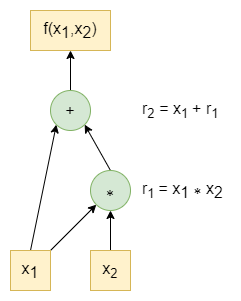
\includegraphics[scale=0.5]{diagrams/forward_example.png}
        \caption{Computational graph of $f(x_1,x_2)\coloneqq x_1+(x_1\times x_2)$}
        \label{fig:forward_graph}
    \end{figure}
    For instance, look at the computational graph in Figure \ref{fig:forward_graph} for $f(x_1,x_2)\coloneqq x_1+(x_1\times x_2)$.
    Now, let us say $x_1=5$, and $x_2=3$, and trace it using the method from Section \ref{sec:tracing}.
    This gives us the trace as \texttt{trace\_result} in Listing \ref{lst:forward_trace}.
    This trace is very straightforward: $x_1$ and $x_2$ are assigned their values, and the multiplication is used in the addition, so it shows up first.
    \begin{haskell}[caption=DSL definition of $f$ and its trace, label=lst:forward_trace, gobble=8]
        f :: Value -> Value -> Expression
        f x1 x2 = ELet "x1" (ELift x1) (
            ELet "x2" (ELift x2) (
                EOp2 Add (ERef "x1") (
                    EOp2 Mul (ERef "x1") (ERef "x2")
                )
            ))

        trace_result :: (TValue, Trace)
        trace_result = (TReal "r2" 20.0, [
            ("x1", TLift (TReal "x1" 5.0)),
            ("x2", TLift (TReal "x2" 3.0)),
            ("r1", TOp2 Mul "x1" "x2"),
            ("r2", TOp2 Add "x1" "r1")
        ])
    \end{haskell}
    Now, let us look at the partial derivatives of $f$ in Equation \ref{eq:reverse_ex}, as we would calculate them using chain rule.
    In Equation \ref{eq:reverse_ex2} we see which calculations we need to perform, we define the partial derivatives or ``adjoints'' of a variable $r_i$ as $\bar{r}_i$.
    We also assume here that the ``seed'' value (the value of $\bar{f}$) is one.
    \begin{equation} \label{eq:reverse_ex}
        \begin{aligned}
            \frac{df}{d\vec{x}}=\nabla f&=\begin{bmatrix}
                \frac{\partial r_2(x_1,r_1)}{\partial x_1}\\
                \frac{\partial r_2(x_1,r_1)}{\partial x_2}
            \end{bmatrix}\tran\\
            &=\begin{bmatrix}
                \frac{\partial x_1}{\partial x_1}+\frac{\partial r_2(x_1,r_1)}{\partial r_1}\cdot\frac{\partial r_1(x_1,x_2)}{\partial x_1}\\
                \frac{\partial x_1}{\partial x_2}+\frac{\partial r_2(x_1,r_1)}{\partial r_1}\cdot\frac{\partial r_1(x_1,x_2)}{\partial x_2}
            \end{bmatrix}\tran\\
            &=\begin{bmatrix}
                1+\frac{\partial r_2(x_1,r_1)}{\partial r_1}\cdot\frac{\partial r_1(x_1,x_2)}{\partial x_1}\\
                0+\frac{\partial r_2(x_1,r_1)}{\partial r_1}\cdot\frac{\partial r_1(x_1,x_2)}{\partial x_2}
            \end{bmatrix}\tran\\
            &=\begin{bmatrix}
                1+1\cdot\frac{\partial r_1(x_1,x_2)}{\partial x_1}\\
                0+1\cdot\frac{\partial r_1(x_1,x_2)}{\partial x_2}
            \end{bmatrix}\tran\\
            &=\begin{bmatrix}
                1+x_2\\
                x_1
            \end{bmatrix}\tran
        \end{aligned}
    \end{equation}
    \begin{equation} \label{eq:reverse_ex2}
        \begin{aligned}
            \bar{f}=\bar{r}_2&=1\\
            \bar{r}_1&=\bar{r}_2\times1\\
            \bar{x}_2&=\bar{r}_1\times x_1\\
            \bar{x}_1&=\bar{r}_2\times1\\
            &+\bar{r}_1\times x_2
        \end{aligned}
    \end{equation}
    With our trace and derivative operations defined, we can now look at how we would get from one to the other.
    It is important to start at the output of the program, and since the trace function we defined in Section \ref{sec:tracing} provides us with the named output, we know where to start on our reverse pass.
    In this case, that would be $r_2$.
    As the final value in the primal calculation is the output of the program, its adjoint will be equal to the adjoint of the program or the seed value.
    This is why Equation \ref{eq:reverse_ex2} posits $\bar{f}=\bar{r}_2$.

    Since we are currently working in reverse execution order, we can just use $\bar{r}_2$ to calculate $\bar{x}_1$ and $\bar{r}_1$ directly.
    It should be reiterated that the trace does not encode any explicit information on the order of operations taken while tracing.
    It is of course a list that was built up one operation at the time, but relying on this forces us to do our reverse pass linearly through the trace, which would prevent some task parallelism opportunities.
    Furthermore, while we can also deduce some order from the naming of the intermediate steps (e.g. $r_1$ was done before $r_2$), we should not do this programmatically, because we wish to reserve parallelism opportunities, but also because some intermediate steps might be hidden in the sub-trace of a map.
    Luckily, we can also discover the ``ancestors'' of any step in the trace by looking at the traced operation.
    For $r_2$ the traced operation was \texttt{TOp2 Add "x1" "r1"}, so we know that for our reverse pass, we next want to look at $x_1$ and $r_1$, as their adjoints (or part of them) rely on the value of $\bar{r}_2$ (which we can also see in Equation \ref{eq:reverse_ex2}).
    For now, we will gloss over how we decide which ancestor adjoint to compute first, and just look at the adjoint of $r_1$.
    
    We know that $\bar{r}_1$ is dependent on $\bar{r}_2$, but how exactly is defined by the operation that produced $r_2$, which in this case is addition.
    Now, addition is really simple, as the derivative of addition of two values is the addition of the derivatives of those values.
    See Equation \ref{eq:reverse_add}, where we calculate the adjoint $\bar{r}_1$ and see how this addition just resolves to $1$.
    \begin{equation} \label{eq:reverse_add}
        \begin{aligned}
            \bar{r}_1&=\bar{r}_2\cdot\frac{\partial r_2(x_1, r_1)}{\partial r_1}\\
            &=\bar{r}_2\cdot\frac{\partial(x_1+r_1)}{\partial r_1}\\
            &=\bar{r}_2\cdot\left(\frac{\partial x_1}{\partial r_1}+\frac{\partial r_1(x_1,x_2)}{\partial r_1}\right)\\
            &=\bar{r}_2\cdot(0+1)\\
            &=\bar{r}_2
        \end{aligned}
    \end{equation}

    We can again find the ancestors of $r_1$ by looking at the trace, where we find $x_1$ and $x_2$.
    Let us look at $x_2$ first.
    $\bar{x}_2$ is dependent on $\bar{r}_1$, which we just calculated, but rather than an addition (like $r_2$), $r_1$ is a multiplication.
    We mentioned in Section \ref{sec:bg_ad}, in Equation \ref{eq:dualnumbers}, how the derivative of a multiplication uses both the primal part and the derivative part of a number.
    To get $\bar{x}_2$ we realize (as is visible in Equation \ref{eq:reverse_ex2} as well), that we need the primal value of $x_1$.
    We mentioned before we needed the intermediate values, and this is why.
    Multiplication is not the only operation that requires a primal component, but it is a prime example.
    We see in Equation \ref{eq:reverse_mul} how this adjoint resolves to use the primal component $x_1$.
    \begin{equation} \label{eq:reverse_mul}
        \begin{aligned}
            \bar{x}_2&=\bar{r}_1\cdot\frac{\partial r_1(x_1,x_2)}{\partial x_2}\\
            &=\bar{r}_1\cdot\frac{\partial(x_1\cdot x_2)}{\partial x_2}\\
            &=\bar{r}_1\cdot x_1
        \end{aligned}
    \end{equation}

    Now would also be a good time to quickly reflect on the difference between the tangent (from forward-mode AD) and the adjoint.
    In forward-mode AD, the operation taken to produce some variable, would influence the tangent of that variable.
    This is somewhat intuitive, $r_1$ is a multiplication, and its tangent is $\dot{r_1}=\dot{x_1}\times x_2+\dot{x_2}\times x_1$.
    However, this is not the case for reverse-mode AD.
    In reverse-mode, we see that this information gets passed on to the adjoints of the variable used by the operation, rather than the variable it produced.
    It should be clear why: the tangents denote how the variable is influenced by a change in the inputs, while an adjoint denotes how its corresponding variable influences the outputs.
    It is important to closely observe this, mainly for implementation purposes: we want to calculate (part of) the adjoint before we actually arrive at that step in the trace.
    To calculate $\bar{x}_2$ we need to know what variable $x_2$ was multiplied with (namely $x_1$).
    This means that if we do not want to search through our trace looking for references (to $x_2$ for example) every time, it would be better to calculate (the relevant part of) $\bar{x}_2$ while we still see how it is being used.\\
    This then also bring us neatly to our next conundrum: what if a variable is used multiple times.
    In the example, this goes for $x_1$, something that we have ignored until now.
    The mathematical solution is simple: the partial derivative of a variable that is used multiple times, is just a summation of the adjoints arising from those uses.
    We see this in Equation \ref{eq:reverse_ex2}, where $\bar{x}_1$ is calculated by adding the influence from $r_1$ and the influence from $r_2$ together.
    However, implementation-wise this can be a bit of a hurdle.

    As mentioned, the trace is not in any order.
    This is unlike a typical Wengert list or tape.
    While assuring some order beforehand, or doing topological sort on the computational graph described by the trace, will in large part solve this problem, it also enforces linear execution of the reverse pass.
    And while it is not something we will linger on for now, allowing for concurrency or task parallelism while calculating the derivative might be a nice for a performance boost, and complement the inherent data-parallelism opportunities of array operations.
    So, to solve this, we want to include some form of reference counting.
    During the forward pass we could count how many times each variable is used in the trace.
    Since we need to store intermediate values anyway, keeping a counter for each of these variables seems like little extra work.
    Now, on the reverse pass we can check these reference counters and every time we find part of the adjoint for a variable, we decrement its associated counter.
    If a counter has not reached zero after we have decremented it, we know its adjoint is not yet complete, and we can ignore it for now.
    If it has, we can add up all the parts of the adjoint and continue from there.
    This is actually very similar to Kahn's algorithm for topological sorting\cite{kahn1962topological}, except that rather than sorting the graph beforehand, we immediately process the nodes as they become available (have all their incoming adjoints).
    This means we actually do execute the reverse pass in topological order, but by discovering this order as we go it allows us to not strictly do the reverse pass sequentially, something of which we will discuss the merits of further on.
    Provided there is only one output to the program, we know that all reference counters will eventually reach zero, and therefore we are assured we will calculate all adjoints.
    However, this provision is not as clear-cut as it seems.
    Currently, our DSL does not really have any room for multiple outputs, and as it is functional does not support any side effects.
    Instead, to provide multiple outputs, currently the only way is to output an array.
    If we keep arrays in the trace, an array as output would still count as a single value.
    There is a slight discrepancy between the trace and the output if we trace away arrays however: the program will still output an array, but only its individual items are present in the trace.
    This is not really a big problem, since the name of these individual outputs are derived from the name of the full array, but also because it would make little sense to trace away arrays from a program that outputs an array.

    So, we find that our trace needs to be extended with two additional things in the forward pass: intermediate values and reference counters.
    We do this in Listing \ref{lst:forward}, in the data type \texttt{Forward}.
    Also, we introduce a clone of the \texttt{Traced} data type as \texttt{Forwarded}, as we need to reference the new \texttt{Forward} type in the constructors for maps and vectorized maps.
    We also replace the list structure of \texttt{Trace} with a key-value map.
    This is not strictly necessary, but it allows us to more quickly access the values in the map, while also clearly communicating there is no pre-set order to the trace.
    Each value in a \texttt{Forward} map is a 3-tuple consisting of respectively: the intermediate value, the traced operation performed, and the reference counter for this variable.
    Other than the added reference counting, and saving of intermediate values, the tracing process remains the same as it was in Section \ref{sec:tracing}.

    \begin{haskell}[caption=Forward pass data structures, label=lst:forward, gobble=8]
        data Forwarded
            = FLift TValue
            | FOp0   Op0
            | FOp1   Op1       String
            | FOp2   Op2       String String
            | FMap   [Forward] String
            | FMapV  Forward   String
            | FFold  Forward   String String
            | FFoldV Forward   String Forward String String

        type Forward = Map String (TValue, Forwarded, Int)
    \end{haskell}

    \subsection{The Reverse Pass}
        As discussed, to facilitate our reverse pass we need both the reference counting and intermediate values.
        Now let us define a function \texttt{reverse} that does the reverse pass.
        This reverse pass should find all the adjoints in the program.
        So, it should take in an object of the \texttt{Forward} type and output a map containing the adjoints.
        In Listing \ref{lst:reverse_def} we define three constructors for adjoints: one for arrays, one for sparse arrays (represented by a single index and the associated value), and one for real values.
        We also define the \texttt{Reverse} type, which will contain these adjoints, and which is returned at the end of the reverse pass.
        The \texttt{Reverse} type maps the names of each part of the calculation to a 2-tuple containing a list of contributions of other adjoints, and its own final adjoint which uses maybe to indicate whether it has been calculated yet.

        \begin{haskell}[caption=Definition of the \texttt{Adjoint} type, label=lst:reverse_def, gobble=12]
            data Adjoint
                = AArray  [Float]
                | AReal   Float
                | ASparse Int Float

            type Reverse = Map String ([Adjoint], Maybe Adjoint)
        \end{haskell}

        Now before going into precise implementation details we should look at the general picture once more.
        The forward pass provides us with three important components: the final output value of the forward evaluation, the trace on which to do our reverse pass, and the intermediate values we will need to actually calculate everything in the reverse pass.
        First off, the final output value is not actually important for the trace, were it not that it also stores its name in the constructor (for \texttt{TValue}, see Listings \ref{lst:traced} and \ref{lst:language_array}).
        This name points us where to start with the reverse pass, namely the step that produced this output value.

        With our starting point clear, we can now start the reverse pass.
        The programmer will provide some sort of adjoint value (either a real number or an array of them, depending on the output of the regular program), which we will immediately assign to our output value in the reverse pass.
        This makes us ready to actually perform the rest of the reverse pass.

        For any point in the reverse pass the process becomes simple.
        Given some ``current'' point in the computational graph, we look up the adjoint (which should have been established by now) and the forward trace item for this point.
        If the operation in the trace for the current point uses no other values (i.e. has no ``ancestors''), we are done here and return the reverse mapping that contains all the adjoints we have found.
        If the operation does have ancestors, we look at the operation itself to determine how to transform the current point's adjoint for its ancestors.
        Then, if this transformation requires any intermediate values, we can look them up in the forward pass.
        Given the transformed adjoints, we assign these to the adjoint accumulation list for each ancestor.
        We also check if this list now has enough adjoints to match the reference counter in the forward pass.
        If it does not, we are done and can return the reverse mapping.
        However, if it does, we add up all the partial adjoints in the list together into the final adjoint and place it in the reverse mapping.
        Then finally, we start the same process for each ancestor of the current node that has its complete adjoint ready.

        Now, let us talk implementation.
        We define two reverse pass functions, \texttt{reverse} and \texttt{resolve}, of which the first will only be a wrapper for the final value and its adjoint to be inserted, and the latter will actually perform the reverse pass.
        Both are shown in Listing \ref{lst:reverse_func}.
        Listing \ref{lst:reverse_func} also introduces two helper functions: \texttt{combineAdjoints} for adding partial adjoints together into the final adjoint of a step in the computational graph, and \texttt{assignAdjoints} for transforming and assigning the adjoints to the ancestors of the current node.
        We will save the intricate details of \texttt{combineAdjoints} and \texttt{assignAdjoints} for later.
        Finally, we use the \texttt{explore} helper function to try and resolve all the ancestors of the current node as well.

        \begin{haskell}[caption=Definition of the reverse pass functions, label=lst:reverse_func, gobble=12]
            reverse :: String -> Adjoint -> Forward -> Reverse
            reverse s a f = resolve s f $\$$ Map.singleton s ([a], Nothing)

            resolve :: String -> Forward -> Reverse -> Reverse
            resolve s f r = case Map.lookup s r of
                -- Lookup the state of the provided name in the reverse mapping
                -- If its present, but its final adjoint not calculated, we need to check
                -- if we can calculate it
                Just (as, Nothing) -> case Map.lookup s f of
                    -- Find the step taken and the reference counter in the forward pass
                    -- If it is present, check whether or not the adjoint array contains
                    -- items equal to the reference counter (so we know it is all there).
                    Just (fd, c, _) -> if   length as >= c
                                       -- If all partials are present, make the complete
                                       -- adjoint and update the reverse map
                                       then let (a,  r1) = combineAdjoints s f r
                                            -- Then transform and assign the adjoints to
                                            -- the ancestors of this current node.
                                                (r2, sa) = assignAdjoints fd s a f r1
                                            -- Then try all the ancestors as well
                                            in  explore sa r2
                                       -- If we are not ready, just return the current
                                       -- reverse map
                                       else r
                    -- If the named variable isn't present in the forward trace, we've
                    -- got a problem, so we throw an error
                    Nothing         -> error "Variable not in forward trace"
                -- If the adjoint is present, and its final adjoint is already calculated
                -- then we must already be done here, so just return the current reverse
                -- mapping
                Just _             -> r
                -- If the adjoint is missing from the reverse mapping entirely, it is because
                -- we haven't run into it at all yet, so we can also return the reverse mapping
                -- as it is.
                Nothing            -> r
                where
                    -- Applies resolve over a list of ancestors
                    explore :: [String] -> Reverse -> Reverse
                    explore []      r' = r'
                    explore (s':ss) r' = explore ss (resolve s' f r')
        \end{haskell}

        We represent this process on the example program from Figure \ref{fig:forward_graph}, in Figure \ref{fig:reverse_graph}.
        In Figure \ref{fig:reverse_graph} we see the computational graph (forward pass) from Figure \ref{fig:forward_graph} first, as (A).

        Then, with $f=r_2$ as our output value from the forward pass, we can call \texttt{reverse} with some adjoint $a$, the name of $r_2$, and the forward pass we just found to get the reverse graph at (B); this assigns a value to $r_2$ in the reverse map, which we call $r'_2$ in Figure \ref{fig:reverse_graph}.

        As part of the reverse map, $r'_2$ contains two items: a list of partial adjoints (currently only containing $a$), and a final adjoint that has not been calculated yet (so is stored as a \texttt{Nothing}).

        Now we can get into the main loop by calling \texttt{resolve} for $r_2$ with the reverse mapping created by \texttt{reverse}.
        As we can see in graph (C), as we find the partial adjoints $r'_2$ and find that the reference counter in the forward pass is $1=|r'_2|$, we can also call \texttt{combineAdjoints}, which transforms the list of partial adjoints in $r'_2$ to the complete adjoint $a$.

        Then we call \texttt{assignAdjoints} to get graph (D).
        \texttt{assignAdjoints} uses the forward pass to find the ancestors of the current node, in this case $x_1$ and $r_1$, and it also adds the final adjoint of the current node ($r'_2$'s final adjoint is $a$) to their lists of partial adjoints.

        Then \texttt{resolve} on $r_2$ calls \texttt{explore} leading to a \texttt{resolve} call to each of $r_2$'s ancestors, with first up $x_1$ in graph (E).
        However, as we can see from the forward graph (A), we still lack the adjoint from $r_1$ to $x_1$ (highlighted with the red arrow in graph (E)), so we can not resolve $x_1$ yet.

        We leave $x_1$ for later, and this leads us to the resolve call on $r_1$ in graph (F).
        Here we find that $r_1$ does have all its partial adjoints, so we call \texttt{combineAdjoints} to find that the completed adjoint for $r_1$ is also $a$.

        Again, with this adjoint found, we can now call \texttt{assignAdjoints} to bring the adjoint of $r_1$ to its ancestors $x_1$ and $x_2$.
        We will go into how later, but \texttt{assignAdjoints} looks in the forward pass to find that $r_1$ is a multiplication and appropriately transforms $r_1$'s adjoint of $a$ into $a\cdot x_2$ for $x'_1$, and $a\cdot x_1$ for $x'_2$.

        Now in our final steps represented in graph (H), we explore the ancestors of $r_1$, starting with $x_1$.
        We find that we now do have the correct number of partial adjoints for $x_1$, so we can add these together with \texttt{combineAdjoints} to get the final adjoint of $x_1$: $a+a\cdot x_2$.
        Now, after \texttt{combineAdjoints} we call \texttt{assignAdjoints} on $x_1$, however we will find that $x_1$ has no ancestors, which means that $x_1$'s adjoint does not need to be assigned to anything and also that there is no further nodes to explore from $x_1$.

        This means we move back to $r_1$'s explore function, which leads us to $x_2$.
        Here we find again that we can use \texttt{combineAdjoints} to get $x_2$'s final adjoint, and with\\\texttt{assignAdjoints} that $x_2$ has no further ancestors.

        This then moves us back to the end of the explore function in $r_1$, which now finished, returns the updated reverse mapping to the end of the explore function of $r_2$, which also finishes, returning the updated reverse mapping to the original \texttt{reverse} function, and return our reverse pass to the programmer.
        
        \begin{figure}[p]
            \begin{adjustbox}{addcode={\begin{minipage}{\width}}{\caption{%
                Diagram representing the reverse pass process on the example from Figure \ref{fig:forward_graph}.
                }\label{fig:reverse_graph}\end{minipage}},rotate=90,center}
                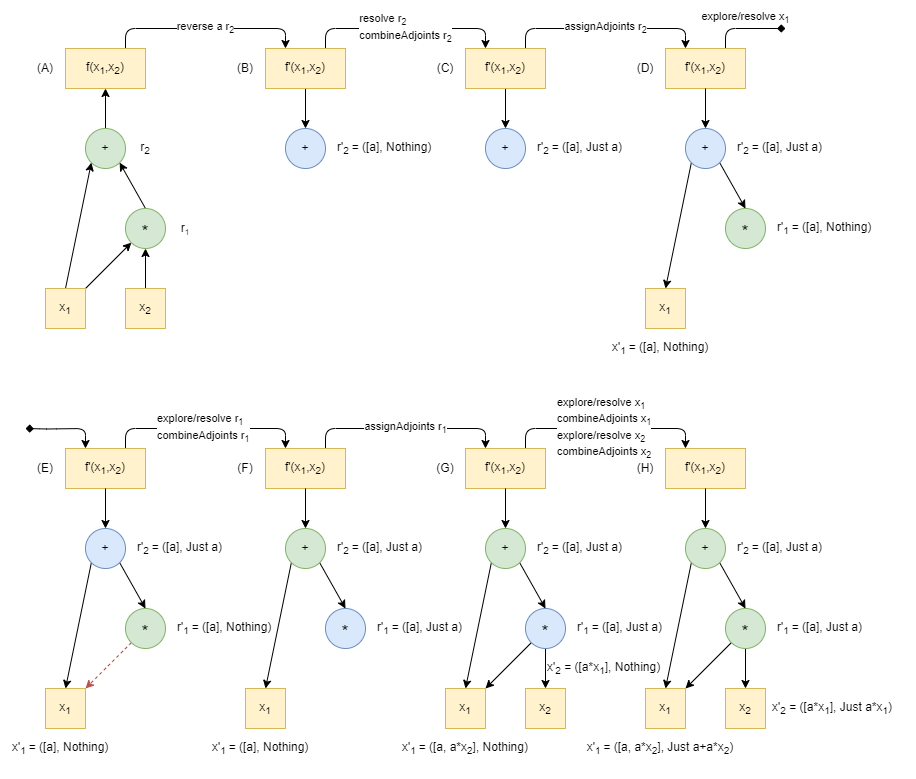
\includegraphics[scale=.6]{diagrams/reverse_example.png}
            \end{adjustbox}
        \end{figure}

        This gives us a global overview of how the reverse pass can be implemented, using the forward pass/trace we have discussed.
        Now there are a couple of questions that remain:
        \begin{itemize}
            \item Can we always add adjoints together?
            \item How do different operations differentiate?
            \item How do we maintain data-parallelism in array operations?
            \item How do we implement task-parallelism on the reverse pass? 
        \end{itemize}
        In the following subsections we will get to all these questions.

    \subsection{Combining Adjoints}
        To go from a list of partial adjoints to a single combined adjoint is not quite as trivial as just adding all together.
        As mentioned before, in Listing \ref{lst:reverse_def}, we defined three types of adjoints, an array, a sparse array, and a real number adjoint.
        The real number adjoint is not complicated, it is the default adjoint, and they can be freely added together.
        The difficulty comes in with the array adjoints.
        These adjoints are produced by operations on arrays.
        It will help us to realize now that the adjoint of an array with length $n$, will also have length $n$.
        In reality the adjoint array is no more than an array of adjoints for each item in the original array.

        Knowing this we can start to discover how to add these adjoints together.
        Let us start by discussing adding the sparse and non-sparse array adjoints, as they are almost as simple as adding two real adjoints.
        Since we only add these together as partial adjoint of a single step in the computational graph, we know that the array adjoints whether sparse or not will always have the same length when added together.
        This means we can just add these arrays of adjoints together element-wise, substituting $0$ for all undefined items in the sparse array.

        Only if we add two sparse arrays together, we might need to look up the length of the original array in the forward pass to know the length of these sparse arrays (or we could extend the sparse array constructor to allow for multiple defined items).

        Now the most interesting part comes when we want to add an array adjoint to a real adjoint, or vice versa.
        Namely, there are two ways of doing this, which means that a binary adjoint addition operator is not associative.
        For example, say we find ourselves folding the values in some array $a$ to some real value $b$.
        In the reverse pass, the adjoint of $b$ will be a real adjoint, yet the adjoint of $a$ will have to be an array adjoint.
        Now provided that $a$ has some partial array adjoint (or is represented by an adjoint array filled with zeroes) we must think of a way to add $b$ to the appropriate items.
        Now what these appropriate items in $a$ are, and how $b$'s adjoint needs to be transformed, are of course dependent on the function we fold over array $a$.

        However, we will find that fold takes in an anonymous function, meaning that we need a special case for fold anyway.
        Only for our unary sum operator we perform a fold that is pre-programmed.
        We know that the sum's result is influenced once by each array item, and from the differentiation rules of addition we know that the adjoint of the sum's result is just moved to its ancestors without transformation or touching intermediate values.
        This means that we can just add the sum's adjoint to each array item.

        The only other way to get from an array to a real value in our language is by using array indexing.
        However, this is very simple as well, as indexing does not change anything to the adjoint either.
        Since indexing refers to a specific item in the array, our partial adjoint for the array becomes a sparse array with the incoming adjoint on the indexed position.

        We see the implementation of the helper function \texttt{combineAdjoints} in Figure \ref{lst:combine}, where we also define a binary adjoint addition operator \lstinline{(<+)} to do most of the heavy lifting.
        It should be reiterated that the \lstinline{(<+)} operation adding a real to an array only works because it will only be called by the sum operator.

        \begin{haskell}[caption=Adjoint combination operator and adjoint summation function, label=lst:combine, gobble=12]
            (<+) :: Adjoint -> Adjoint -> Adjoint
            (<+) (AArray as)   (AArray    bs) = AArray (zipWith (+) as bs)
            -- Note: this works because it is only called by sum
            (<+) (AArray as)   (AReal     bs) = AArray (map (+ b) as)
            (<+) (AArray as)   (ASparse i bs) =
                let bs = drop i as
                in  AArray (take i as ++ (b + head bs) : tail bs)
            (<+) (AReal  a)    (AArray    bs) = AReal (a + sum bs)
            (<+) (AReal  a)    (AReal     b)  = AReal (a + b)
            (<+) (AReal  a)    (ASparse _ b)  = AReal (a + b)
            (<+) (ASparse i a) (AArray    bs) = 
                let as = drop i bs
                in  AArray (take i bs ++ (a + head as) : tail as)
            (<+) (ASparse _ _) (AReal     _)  = error "Cannot combine sparse and real
                adjoints, because the length of the sparse adjoint is unknown."
            (<+) (ASparse _ _) (ASparse _ _)  = error "Cannot combine two sparse adjoints,
                because the length of the sparse adjoints are unknown."

            combineAdjoints :: String -> Forward -> Reverse -> (Adjoint, Reverse)
            combineAdjoints s f r =
                -- Get the partial adjoints and combine them together
                let (as, _) = r Map.! s
                    a       = foldr (<+) empty as
                -- And add the completed adjoint to the reverse map
                in  (a, Map.insert s (as, Just a) r)
                where
                    -- Provide an empty identity element
                    empty :: Adjoint
                    empty = case getValue s f of
                        -- Check the intermediate value of s to reveal the right identity element
                        (FArray _ xs) -> AArray (replicate (length xs) 0.0)
                        (FReal  {})   -> AReal  0.0
                        _             -> error "Type mismatch in combineAdjoints/empty"
        \end{haskell}

    \clearpage
    \subsection{Differentiating Operations}
        The actual differentiation rules are applied in the \texttt{assignAdjoints} function, where we take the complete adjoint of a node in the computational graph, transform it according to the operation performed in that node, and then add it as a partial adjoint to its ancestors.
        It is especially the transformation that means we need to write different differentiation rules for almost every operation.

        Let us start with the easy part, the unary and binary mathematical operators.
        In our DSL these are: addition, multiplication, subtraction, and sine.
        Recall that the rules for addition and subtraction are similar, they just transform homomorphically, which means that any adjoint is just ``passed'' to their ancestors without any additional transformation.
        See the examples in Equation \ref{eq:diff_add}.

        \begin{equation} \label{eq:diff_add}
            \begin{aligned}
                \frac{d(x+y)}{dz}&=\frac{dx}{dz}+\frac{dy}{dz}\\
                \frac{d(x-y)}{dz}&=\frac{dx}{dz}-\frac{dy}{dz}
            \end{aligned}
        \end{equation}

        Multiplication and sine are slightly more complicated, both requiring some intermediate value to compute the derivative.
        We have gone over multiplication before, we multiply the incoming adjoint with intermediate value of the other side of the multiplication.
        See the example in Equation \ref{eq:diff_mul}.

        \begin{equation} \label{eq:diff_mul}
            \frac{d(x\cdot y)}{dz}=y\cdot\frac{dx}{dz}+x\cdot\frac{dy}{dz}
        \end{equation}

        The derivative of a sine operation is the cosine on the intermediate value, see Equation \ref{eq:diff_sin}.

        \begin{equation} \label{eq:diff_sin}
            \frac{d(\sin x)}{dy}=\cos x\cdot\frac{dx}{dy}
        \end{equation}

        These are the mathematical operations that we may encounter in the trace.
        Recall that we traced away Booleans, so we do not have to worry about comparison operators.
        With these derivatives cleared up we can now program them into \texttt{assignAdjoints}.
        It is also useful to remember that \texttt{assignAdjoints} should return both the updated reverse mapping, and a list containing the ancestors of the provided node.
        We see the implementation in Listing \ref{lst:assign_simple}.
        This uses another helper function called \texttt{addAdjoint}, which simply just adds the calculated partial adjoint to the list of partial adjoints of the relevant ancestor in the reverse mapping.

        \begin{haskell}[caption={Defining \texttt{assignAdjoints} for sine, addition, subtraction, and multiplication.}, label=lst:assign_simple, gobble=12]
            assignAdjoints :: Forwarded -> String -> Adjoint -> Forward -> Reverse
                -> (Reverse, [String])
            -- Adjoint function for all unary operators (now only showing sine)
            assignAdjoints (FOp1 op s1) _ a f r = case (op, a) of
                (Sin, AReal a') -> case getValue s1 f of
                    -- Take the intermediate value and assign the adjoint to s1, also return
                    -- the list of ancestors: s1
                    (FReal _ x) -> (addAdjoint s1 (AReal $\$$ a' * cos x) r, [s1])
                    _           -> error "Type mismatch in assignAdjoints/FOp1/Sin"
                _               -> error "Type mismatch in assignAdjoints/FOp1"
            
            -- Adjoint function for all binary operators
            assignAdjoints (FOp2 op s1 s2) _ a f r = case (op, a) of
                -- Just add the adjoint to both ancestors
                (Add, _)        -> (addAdjoint s1 a (addAdjoint s2 a r), [s1, s2])
                -- For multiplication, get the intermediate values first
                -- we also deconstruct the adjoint, knowing it is a real number because
                -- (sin x) would return a real number.
                (Mul, AReal a') -> case (getValue s1 f, getValue s2 f) of
                    (FReal _ v1, FReal _ v2) ->
                        (addAdjoint s1 (AReal (a' * v2)) (addAdjoint s2 (AReal a' * v1) r), 
                        [s1, s2])
                    _                        ->
                        error "Type mismatch in assignAdjoints/FOp2/Mul"
                -- Similar to addition, only s2 gets a negative adjoint
                (Sub, AReal a') -> (addAdjoint s1 a (addAdjoint s2 (AReal -a') r), [s1, s2])
                _               -> error "Type mismatch in assignAdjoints/FOp2"
        \end{haskell}

        Another adjoint we should quickly cover is that of array indexing.
        As mentioned before, nothing happens to an intermediate value when it is indexed, so its adjoint will not be transformed either.
        While obvious, the adjoint of the indexed value should only be added to the that specific index in the array's adjoint.
        This is where our sparse adjoint comes in, where we represent a single item in the array without storing anything extra.
        We can see how it is used by \texttt{assignAdjoints} for indexing in Listing \ref{lst:assign_idx}.

        \begin{haskell}[caption={Defining \texttt{assignAdjoints} for the indexing operation}, label=lst:assign_idx, gobble=12]
            assignAdjoints :: Forwarded -> String -> Adjoint -> Forward -> Reverse
                -> (Reverse, [String])
            assignAdjoints (FOp1 op s1) _ a f r = case (op, a) of
                -- Add the sparse array and return the name of the array as ancestor
                (Idx i, AReal a') -> (addAdjoint s1 (ASparse i a') r, [s1])
                $\dots$
            $\dots$
        \end{haskell}

        \subsubsection{The reverse pass on map operations and function closures}
            Unsurprisingly, the reverse pass is slightly more in-depth on array operations, like map.
            For a regular non-vectorized map, this is still fairly easy to wrap our heads around.
            Especially if we remember that our forward-pass provides us with the following constructor for such maps:
            \lstinline[language=haskell]{FMap [Forward] String}.
            Here we store every application of the mapped function to our array as its own sub-trace.
            Now it becomes easy to realize that the simplest way to reverse-pass over this mapping is just to call the \texttt{reverse} function on each of these forward sub-traces.
            This then provides us immediately with the adjoint of each original array item, which we can combine into an array adjoint for the original array.
            We give this array adjoint as a partial adjoint to the original array (as it is the ancestor of the mapping operation).
            It should be explicitly stated that mapping the \texttt{reverse} function reveals the derivative of a map: another map, but in reverse.

            However, there is a slight obstacle yet to overcome; to do with the mapped function.
            What do we do if the function that is mapped over the array uses variables from anywhere outside the actual array?
            Recall that the functions that are mapped are lambda expressions that have access to any variables in the environment at the function's definition.
            As an example, we can see this expressed in Figure \ref{fig:map_graph}, where some mapped operation on an array $[b]$ uses a variable $a$ to produce the array $[c]$.
            While the partial adjoints for this variable are computed during the reverse pass over every item, they are only stored in the reverse mapping for the particular item.
            And if we extract only the adjoint for the original array item from this reverse mapping, we would throw away these partial adjoints, making it possibly impossible for us to calculate the full reverse-pass of the program, as we will not be able to calculate the adjoint for these outside variables.
            We find that these variables, like $a$ in \ref{fig:map_graph} are ``unofficial ancestors'' of the mapping operation.
            They are used by the mapping operations, but can be a little hard to find, as they are hidden in the sub-traces.

            \begin{figure}[htb]
                \centering
                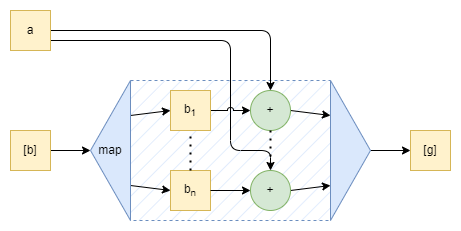
\includegraphics[width=0.6\textwidth]{diagrams/map_example.png}
                \caption{Example of an unofficial ancestor to an array operation}
                \label{fig:map_graph}
            \end{figure}

            Luckily for us the main difficulty with this problem is noticing it.
            Now we know that we have to extract this data into the main reverse pass, we can simply merge the item's reverse pass with the main one.
            We only need to be wary of extracting the partial adjoints for the original map, and combining them together, so we do not over count the number of partial adjoints against the reference counter of the original array (that in the forward pass only got increased by one for use in the map operation.)
            We see the whole process of finding the adjoint of a map in Listing \ref{lst:assign_map}.

            \begin{haskell}[caption=Implementation of \texttt{assignAdjoints} for the map operation, label=lst:assign_map, gobble=16]
                assignAdjoints :: Forwarded -> String -> Adjoint -> Forward -> Reverse
                    -> (Reverse, [String])
                $\dots$
                assignAdjoints (FMap fss s1) s a _ r =
                    let (as, r', ss) = reverseMap fss 0
                        -- Fold sparse adjoints into single array adjoint
                        a' = foldl (<+) (AArray $\$$ replicate (length fss) 0.0) as
                    in  (addAdjoint s1 a' r', Set.toList ss)
                    where
                        reverseMap :: [Forward] -> Int -> ([Adjoint], Reverse, Set String)
                        reverseMap []     _ = ([], r, Set.empty)
                        reverseMap (f:fs) i =
                            let s'  = s ++ '!' : show i
                                rx  = reverse f s' (indexAdjoint i a)
                                -- Extract the array item for 
                                ax  = toSparse i $\$$ fst $\$$ combineAdjoints s' f rx
                                -- Remove items from the original and destination array from this reverse pass
                                -- and add the array items partial adjoint
                                rx' = Map.delete s' (Map.delete (s1 ++ '!' : show i) rx)
                                -- Find the results of the rest of the map
                                (axs, rxs, sxs) = reverseMap fs (i + 1)
                            in  (
                                -- Add this sparse partial to the list
                                ax : axs,
                                -- Add rx' to the main reverse pass
                                Map.unionWith unionReverse rxs rx',
                                -- Add relevant keys to the set of ancestors
                                Set.union sxs $\$$ Map.keysSet rx'
                            )
                        toSparse :: Int -> Adjoint -> Adjoint
                        toSparse i (AReal a') = ASparse i a'
                        toSparse _ _          =
                            error "Type mismatch in assignAdjoints/FMap/toSparse"
            \end{haskell}

            Now with the non-vectorized map taken care of, we can move on to the vectorized map.
            While the idea of finding the adjoint to the map remains the same of course, we now find ourselves with a new problem: a lack of intermediate values.
            Recall that when tracing a vectorized map, we only stored the trace of a single item in the array.
            This was possible because, as we had found the mapped function would not branch, the trace would be the same for each item.
            Now, provided that we did store all intermediate values for this mapping operation, we can perform the same reverse map for the vectorized trace, as with the nonvectorized trace.

            \paragraph*{On map parallelism}\mbox{}\\
                It should be clear that there is a major inherent parallelism opportunity for each of the mapping operations.
                For the vectorized map this is very clear: data parallelism.
                This is true in evaluation, and is still true in the reverse-pass.
                Namely, as the reverse pass is the same for all items, we can use a data parallel mapping function to run the reverse pass in a vectorized manner as well.

                For the non-vectorized map we cannot be sure the operations are the same for each item.
                This means that data parallelism is off the table, however we can still use task parallelism.
                This would not be hard to implement as each item has its own reverse call which can easily be run task parallel.
                Of course, one would need to exercise some caution with the collection of the partial adjoints and reverse maps, but this is not a new problem.
                The combination of the partial adjoints would still need to happen sequentially.

                We will talk more about parallelism when we talk about the reverse map on folds.

        \subsubsection{The reverse pass on fold operations}
            The regular fold operator in our language (for branching functions) is simply implemented as a sequential left-to-right fold.
            This is mainly because we can not reliably apply data parallelism on a function that may behave differently for different elements.
            However, this makes the reverse-pass over such a fold extremely easy, since this operation can be captured in a single forward sub-trace.
            Like what we saw with maps, we can just run our general \texttt{reverse} function over this sub-trace, and find the adjoint for the original array, and the identity element.
            Also like with maps, we can then combine this reverse mapping with the main reverse mapping to make sure we do not lose out of any adjoints for informal ancestors that may arise from the closure on the folding function.
            We see this put into code in Listing \ref{lst:assign_fold}.

            \begin{haskell}[caption=Reverse pass over a sequential fold, label=lst:assign_fold, gobble=16]
                assignAdjoints :: Forwarded -> String -> Adjoint -> Forward -> Reverse
                    -> (Reverse, [String])
                $\dots$
                assignAdjoints (FFold f s1 s2) s a _ r =
                        -- Get the reverse mapping
                    let rf = reverse f s a
                        -- Extract the adjoint for the array and the identity elements
                        aa = fromJust $\$$ snd $\$$ rf Map.! s1
                        az = fromJust $\$$ snd $\$$ rf Map.! s2
                        -- Combine the reverse map with the main reverse map
                        r' = Map.unionWith unionReverse r (Map.delete s1 (Map.delete s2 rf))
                    in  (addAdjoint s1 aa (addAdjoint s2 az), [s1, s2])
            \end{haskell}

            As discussed, our vectorized fold operation uses a segmented fold followed by a sequential fold.
            Of course if we have more threads available than we have items in our array, we use a sequential fold instead.
            Since in the reverse-pass we pass over the second step before the first step, it is important to recall that to properly gather the results from the first step sub-traces, we use an \texttt{FJoin} constructor, which we can use in the reverse pass to pass the adjoints back to the correct sub-trace.
            We can see this all come together in the implementation in Listing \ref{lst:assign_foldv}.

            Of course, when we encounter the \texttt{FJoin} constructor in the reverse pass, we still need to apply the reverse-pass on it.
            However, since the \texttt{FJoin} is not a real numerical operation, it also has no derivative.
            So we just ignore \texttt{FJoin}, as it is the starting point for the second step anyway, it has no values depending on its derivative.
            The derivative it does get is an array containing derivatives for the joined values (from the first step), to be used in the reverse-pass for the first step.
            
            \begin{haskell}[caption=Reverse pass over a vectorized fold, label=lst:assign_foldv, gobble=16]
                assignAdjoints :: Forwarded -> String -> Adjoint -> Forward -> Reverse
                    -> (Reverse, [String])
                $\dots$
                assignAdjoints (FFoldV f1 q f2 s1 s2) s a _ r =
                    if   Map.null f2
                    -- If the forward pass for step 2 is empty, we used a sequential fold
                    then let rf = reverse f1 s a
                             -- Extract the adjoint for the array and the identity elements
                             aa = fromJust $\$$ snd $\$$ rf Map.! s1
                             az = fromJust $\$$ snd $\$$ rf Map.! s2
                             -- Combine the reverse map with the main reverse map
                             r' = Map.unionWith unionReverse r 
                                (Map.delete s1 (Map.delete s2 rf))
                         in  (addAdjoint s1 aa (addAdjoint s2 az), [s1, s2])
                    -- If not we are dealing with a proper vectorized fold
                             -- Reverse pass over the second step first
                    else let r2 = reverse f2 s a
                             -- Extract the adjoint for the join from step 2
                             a2 = fromJust $\$$ snd $\$$ r2 Map.! q
                             -- Combine the reverse map for step 2 with the main one
                             r' = Map.unionWith unionReverse r (Map.delete q r2)
                             -- Get the join's contents
                             ss = getJoin
                             -- Get the update reverse mapping, the partial adjoints of the array,
                             -- and the adjoint of the identity element.
                             (r'', a1s, z') = getParts ss (fromJust a2) r'
                             -- Combine the partial adjoints for the array into one
                             a1 = foldl (<+) (AArray $\$$ replicate (Map.size f1) 0.0) a1s
                         in  (addAdjoint s1 a1 (addAdjoint s2 z' r''), [s1, s2])
                    where
                        getJoin :: [String]
                        getJoin = case f2 Map.! q of
                            (FJoin ss, _, _) -> ss
                            _                -> error "Type mismatch in assignAdjoints/FFoldV"
                        
                        -- Get the updated reverse mapping, the adjoint for the array,
                        -- and the adjoint for the identity element
                        getParts :: [String] -> Adjoint -> Reverse 
                            -> (Reverse, [Adjoint], Adjoint)
                        getParts []      _                rv = (rv, [], AReal 0.0)
                        getParts (s':ss) (AArray (a':as)) rv =
                            let rx = reverse f1 s' (AReal a')
                                ax = fromJust $\$$ snd $\$$ rx Map.! s'
                                (rxs, axs, zxs) = getParts
                                rx' = Map.unionWith rxs (Map.delete s1 (Map.delete s2 rx))
                            in  case Map.lookup s2 rx of
                                -- Update the adjoint for the identity element only if it was used
                                -- by this segment.
                                Just (zs, _) -> (rx', ax : axs, foldl (<+) zxs zs)
                                Nothing      -> (rx', ax : axs, zxs)
            \end{haskell}

            \paragraph{On the sum operation}\mbox{}\\
                The DSL implements a special kind of fold as a unary operator, namely the sum operation.
                Recalling that the sum operator just adds up the values in an array, we can implement this as a fold over the array, using the addition operator and $0$ as the identity element.
                However, the reverse pass over a sum operation is very simple.
                Starting with some real adjoint $a$ at the result of the sum, this adjoint is then passed through all the addition operators to all the members of the original array.
                This allows us to quickly make the adjoint for the original array, namely an array adjoint where all values are $a$.
                Taking such a shortcut also means leaving out the adjoints for all intermediate calculations, however since we intuitively know what they are for sum, this should not really pose a problem.
                In Listing \ref{lst:assign_sum} we see the implementation of the \texttt{assignAdjoints} function for the sum operation.

                The main takeaway here is not really about sum, however.
                It is that special cases exist in the reverse pass, even if they seem somewhat generic in the regular program.
                Finding these special cases can increase the speed of the reverse pass.
                While the sum operation might not be too exciting an example, it highlights that we should be on the lookout for these special cases, especially for the more complex ones (as they will profit more from the potential speed-up.)

                \begin{haskell}[caption=Implementation of the sum operator in \texttt{assignAdjoints}, label=lst:assign_sum, gobble=20]
                    assignAdjoints :: Forwarded -> String -> Adjoint -> Forward -> Reverse
                        -> (Reverse, [String])
                    $\dots$
                    assignAdjoints (FOp1 op s1) _ a f r = case (op, a) of
                        $\dots$
                                           -- We need to get the arrays length for the adjoint
                        (Sum, AReal a') -> case getValue s1 f of
                            (FArray _ xs) ->
                                (addAdjoint s1 (AArray $\$$ replicate (length xs) a') r, [s1])
                            _             -> error "Type mismatch in assignAdjoints/FOp1/Sum"
                    $\dots$
                \end{haskell}

            \paragraph{On fold parallelism}\mbox{}\\
                Fold parallelism is also a little more complicated than map parallelism.
                An easy way to think about why, is by visualizing the flow of data in both operations.
                In map, we start with an array of $n$ items, and end with one.
                Every array element ``flows'' from some index in our original array to the same index in the resulting array, never intersecting with any of the other elements.
                With folding operations, it is especially this intersection of the dataflows that makes it hard to parallelize in the reverse pass.
                If we imagine the values in the original array as being funnelled into the final result, we quickly realize that there is no operation that does the opposite: there is no ``unfold'' operation.
                However, both the individual segments in the first step of the fold, and the combination in the second step are relatively simple sequential folds.
                While the intermediate values in a folding operation are ignored in regular use, we actually store them as part of our forward traces.
                This means that our sequential folds are more like a scan, a left-to-right scan to be precise.
                Realizing this, we can imagine our reverse-pass as a right-to-left scan, applying the fold (or calculating its adjoints) in reverse if you will.
                Of course this works on sequential fold, but it works on the data-parallel fold as well, and we can maintain almost the same parallelism as before.
                First, we calculate the adjoints in the second step using a sequential right-to-left scan, and then we do the same for the segments in the first step, now in parallel.
                Of course, the resulting adjoint arrays of each segment would still need to be combined sequentially, which is not necessary in the regular fold.
                Still, this preserves the data-parallelism present in the fold, which was our goal.
            
    \subsection{Task parallelism in the reverse pass}
        We have paid some attention to data parallelism for data parallel operations, namely map and fold.
        However, we can also more generally implement task parallelism on the reverse pass as a whole.
        This is mainly why we have previously been adamant about not sorting the array, and having unique but non-sequential names (they may in fact be sequential, but should not be treated as such): it means we can execute the reverse pass in any order as long as we make sure to keep an eye out for missing partial adjoints.
        Again, we compare the number of collected partial adjoints of a computational step, to the number of references made to that step (according to the forward pass), and we only combine the adjoints if they match.
        This way we know we do not calculate the step's adjoint prematurely, but we also know that if we cannot calculate the adjoint, another part of the reverse pass will, as it will provide the last piece of that adjoint.

        Eventually this comes together in the fact that we may perform the reverse pass completely asynchronously.
        We start with one thread at the end of the computation, but whenever part of the computation assigns adjoints to multiple ancestors, we can check these ancestors using task parallelism.
        We can just spawn new threads to deal with all but one ancestor, and continue the original thread on the remaining ancestor, and combine results back into the final result later.
        For large or complex traces this might actually allow us to significantly speed up our reverse pass.

        It should be noted that our current implementation does not quite allow for this kind of task parallelism, because right now it returns the reverse mapping back to the starting point, meaning that the through-putting of the reverse mapping from one ancestor to the next forces sequential execution.
        However, this can easily be fixed using a mutable variation of the reverse mapping.
        While this would violate purity (which does not allow for mutable variables), the speed-up might be worth it.

    \subsection{Finding Complexity}
        With now the reverse pass figured out, we can start talking about estimating a time complexity for this program.
        We will try to do so with regard to the execution time of the regular program, which we will denote with $n$, where $n$ is a stand-in for the number of steps in our execution graph.
        This means that regardless of the functions actual complexity, for this section the complexity of executing a function consisting of $n$-substeps, would have a complexity of $O(n)$.

        For the forward pass we find that any recording of references to reference counters, or storing intermediate values should only provide us with a small overhead on the regular execution of the program.
        After all, we only count direct references, and we already have to calculate the intermediate values for execution anyway, storing them is not much of a problem.
        Of course, we do gain some time complexity overhead depending on the storage method.
        For tracing we used a built-in Haskell list, which can store new items in $O(1)$ time.
        However, for ease of use, we switched to a map (associative array) when we expanded to the forward pass.
        While of course lookup and getting in a map of size $m$ is quicker than in an list of size $m$ ($O(\log m)$ as opposed to $O(m)$), insertion on a map also takes $O(\log m)$ time.
        This means that we can assume our forward pass roughly takes $O(n\log n)$ time: for $n$ steps in the execution, we record intermediate values at the cost of $O(\log n)$ time

        Of course, this overhead in the forward pass, allows us to safe a little time in the reverse pass.
        Let us assume that for each step in our reverse pass, we need to retrieve the intermediate value at a cost of $O(\log n)$.
        Furthermore, we also need to write a partial adjoint to each ancestor of the step.
        Since we store these (partial) adjoints in a map as well, we know this will take $O(\log n)$ time to store for each ancestor.
        Luckily for us, each operation has only at most three ancestors, so we can still keep this overhead at $O(\log n)$.

        Unfortunately, not all can currently be covered in a $O(\log n)$ overhead, because of the array operations.
        After finishing a map or fold operation, we need to join the reverse passes over the sub-traces back into the main trace.
        This union operation takes $O(m)$ time, where $m$ is the size of the smaller map.
        There are two ways to remedy this however.
        First, we could make the reverse mapping a mutable variable.
        This way we can write new adjoints to the main reverse mapping directly, meaning we do not need to do any union operations.
        In a similar vein we could write a special reverse function for sub traces like this, that produce a new reverse mapping based on what happened in the sub-traces, while keeping the main trace up until that point intact.
        This means we can maintain purity, however it also means that we can not parallelize, as every sub-trace would need the reverse mapping of the previous sub-trace.
        (Or we could union these sub-trace reverse mappings again, but that would bring us back to the problem of union's time complexity.)

        Regardless of how we wish to solve it, the current time complexity of the overhead produced by these operations is $O(n)$, meaning the time complexity of the reverse map becomes $O(n^2)$.
        When allowing mutability on the reverse mapping we could bring this down to an $O(\log n)$ overhead, or a time complexity of $O(n\log n)$.
        
        This brings the total time complexity of the whole AD process as described to $O(n^2+n\log n)\approx O(n^2)$, which is not great.
        However, we can also see that this overhead occurs due to implementation details.
        For instance, in general we would describe the insertion and lookup complexity of an associative array (with size $m$) as $O(1)$ rather than $O(\log m)$, which eliminates these logarithmic overheads from the run altogether.
        However, due to implementation details in the mapping (provided by the containers package in Haskell), this turns out to be $O(\log m)$.
        Also, for the unions, we claim an $O(n)$ overhead, which is truly the worst case, assuming that all adjoints are already present in the reverse mapping (but we somehow need to add some more).
        Generally (and ideally), the reverse mappings for these sub-traces would be much smaller than those of the main reverse mapping, meaning a smaller overhead as well.
        If we assume the largest of these sub-trace reverse mappings has some size $k\ll n$, and we use the regular insert/lookup time complexity of $O(1)$, we find an idealized time complexity of $O(nk+n)$, which is much closer to the optimal time complexity $O(n)$ (as the complexity of the reverse-pass is ideally upper-bounded by $6\cdot n$).

        Finally, the speed-up we expect from task and data parallelism is wholly dependent on the shape of the computational graph, and the number of threads we can run simultaneously.
        For task parallelism, the ideal shape of the computational graph would be a tree (with the final result as the root), because it will allow us to make use of as much task parallelism as possible, without running into dead ends (due to missing partial adjoints).
        Similarly, data parallelism provides great advantage for vectorizable operations on large arrays.
        Of course, this dependency on the shape of the program means we cannot make a general statement about how these speed-ups would actually translate to time complexity.
        
        It should be noted though, that especially data-parallelism has been left by the wayside by the large AD libraries, in favour of machine parallelism (where data and instructions are separated over multiple machines).
        While theoretically more scalable than regular data parallelism, machine parallelism is useful mostly for specific use cases like machine learning, and is also financially more costly.
        This means that machine parallelism is mostly reserved for large companies who can leverage multiple machines or even data centres to do this, while leaving groups with less resources out in the cold somewhat.